\contribution{The Vector Execute Units}
\shortcontributor{CS6230 : CAD for VLSI Project Report}
\shortcontribution{Vector Extensions}
\headnum{8}
\begin{paper}
\renewcommand*{\pagemark}{}

\section*{}
The data from the temporary storage units arrive at the right execute units designated by the Opcode through a Pipeline FIFO. The architecture of the two main vector functions that we focus on in this project is given below.
\section*{Vector Negation\sdot}
Implementing elementwise vector negation was relatively straight forward as there is only one to one correspondence between the inputs and outputs. For integers in 2's complement representation, negation is achieved by inverting all numbers and adding one. However, the abstraction level provided by the implementation of integers in Bluespec libraries hides all details from the writer and can be written directly. \\\\
\nointend For floating-point values, merely flipping the sign bit of a value results in the number's negative. We employed Bluespec's \texttt{FloatingPoint} library, which provided direct arithmetic functionality.
\section*{Vector Statistics Minima\sdot}
The statistics minima operation is devised to run in logarithmic time complexity. Since every vector is of variable length, usually longer than the execution unit's width, we were required to maintain the system's state. The state contains the value of the minimum from the previous batch. The state is updated if the current batch's minimum is less than the minimum of the previous batch. A status signal of 'Break' resets the states. The indices of the minima are also calculated concurrently along with the minima.
\begin{figure}[H]
\centering
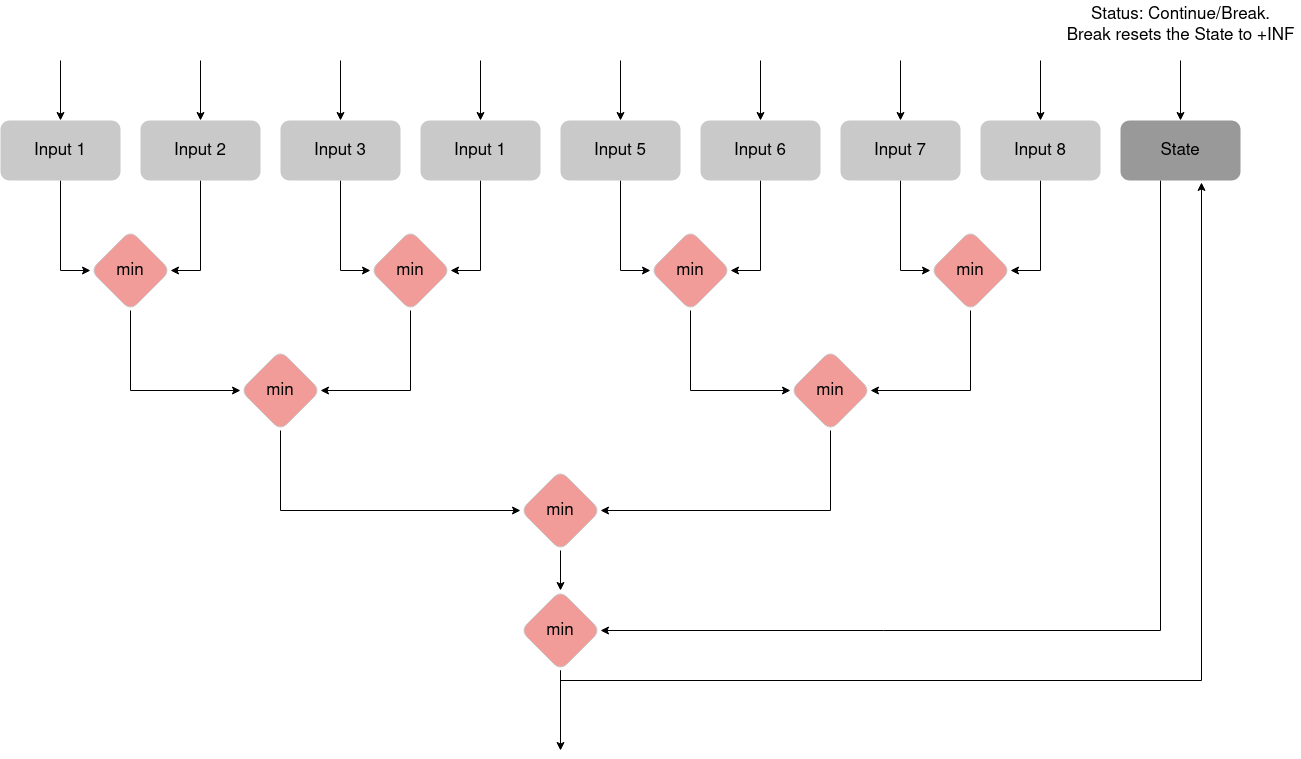
\includegraphics[width=\textwidth]{Images/VectorExtensions-minima.png}
\caption{\content Execute unit for computing statistics minima.}
\end{figure}


\end{paper}